\documentclass[11pt]{article}
\usepackage[utf8]{inputenc}
\usepackage[T1]{fontenc} 
\usepackage[french]{babel}
\usepackage{graphicx}
\usepackage{subcaption}
\usepackage[table]{xcolor}
\usepackage{longtable}
\usepackage{geometry}

\begin{document}

\tableofcontents
\newpage

\section{Etat de l'art}\label{sec:eda}
	Avant d'apporter une contribution à notre projet, et plus particulièrement à la problématique de l'ingestion de données en temps-réel provenant de capteurs, nous devons nous intéresser à ce qu'il existe dans la littérature scientifique et technique actuelle. 
	Pour cela, nous nous sommes intéressés aux approches permettant l'adaptation de jeux aux états émotionnels et à d'autres caractéristiques des joueurs.
	Pour comparer et évaluer ces approches, nous avons élaboré notre propre cadre de comparison.
	Ce cadre nous permet de distinguer différents points clés qui vont nous permettre d'apporter une réponse à notre problématique et qui vont nous aider à la réalisation de notre projet.\par
	Dans cette section, nous présentons dans un premier temps le cadre de comparaison que nous avons mis au point.
	Et dans un second temps, nous appliquons ce cadre à plusieurs approches que nous avons relevées afin de faire ressortir des méthodes qui pourront nous être utiles pour apporter une contribution pour ce projet.
	\subsection{Cadre de comparaison}\label{sec:edacadre}
		Nous cherchous à comparer des approches traitant de l'adaptation dynamique de jeux pervasifs aux états émotionnels et à d'autres caractéristiques des joueurs.
		Pour cela, nous devons nous appuyer sur une comparaison commune entre toutes les approches.
		Nous avons donc élaboré notre propre cadre de comparaison. 
		Ce cadre nous permet d'avoir une vue d'ensemble sur la façon dont l'adaptation est traitée par les méthodes comparées.\par
		Pour comparer et évaluer les approches que nous avons sélectionnées pour ce rapport, mais également pour de futures recherches, notre cadre s'appuie sur les critères suivants :
		\begin{itemize}
			\item Les méthodes pour la détection et pour la reconnaissance des états émotionnels
			\begin{itemize}
				\item Les capteurs utilisés
				\item Les algorithmes utlisés pour la détection et/ou la reconnaissance de l'état émotionnel
			\end{itemize}
			\item Les autres caractéristiques de l'utilisateur prises en compte par le jeu
			\item Les méthodes d'adaptation d'un jeu au contexte de son utilisateur
			\begin{itemize}
				\item Les méthodes pour l'adaptation du jeu selon l'état émotionnel du joueur
				\item Les méthodes pour l'adaptation du jeu selon d'autres caractéristiques du joueur
			\end{itemize}
		\end{itemize}\par
		Le critère "méthodes pour la détection et pour la reconnaissance des états émotionnels" nous permet d'identifier d'une part les capteurs utilisés (s'ils existent).
		Et d'autre part, les algorithmes utilisés pour la détection et la reconnaissance d'états émotionnels.
		Comme nous visons à utiliser des capteurs pour notre projet, il est important pour nous de savoir si certains capteurs reviennent souvent dans la littérature et s'ils sont performants pour ce type d'application.
		Nous visons aussi à utiliser des algorithmes d'apprentissage profond non-supervisés pour la reconnaissance d'états émotionnels (comme celui décrit dans \cite{gal_et_al._2020}), alors nous avons cherché à savoir s'il existait déjà des algorithmes similaires.\par
		Le critère "autres caractéristiques de l'utilisateur prises en compte par le jeu" nous permet d'identifier s'il existe d'autres données que celles concernant l'état émotionnel pour une "bonne" adaptation d'un jeu.
		Ce critère permet d'élargir notre champ de recherche.\par
		Le dernier critère "méthodes d'adaptation d'un jeu au contexte de son utilisateur" permet d'identifier les algorithmes pour l'adaptation dynamique et particularisée d'un jeu.
		D'un côté nous explorons les algorithmes utilisant l'état émotionnel du joueur.
		Et de l'autre, nous explorons les algorithmes utilisant d'autres caractéristiques du joueur.
		Comme nous souhaitons que notre jeu soit particularisé à chaque joueur et que l'adaptation se fasse en temps-réel, nous cherchons des approches qui utilisent ce genre d'algorithmes.
		Nous nous intéressons tout particulièrement aux approches qui présentent des algorithmes pour l'adaptation dynamique aux états émotionnels des joueurs.\par
		Ce cadre peut être appliqué à des recherches scientifiques et à des jeux déjà existants sur le marché.
		Pour notre état de l'art, nous avons appliqué notre cadre à douze approches différentes.
		Ces approches concernent différents types de jeux (jeux sérieux, jeux-vidéo, jeux pervasifs,...).
	\subsection{Application du cadre}\label{sec:appcadre}
		Pour cette état de l'art, nous avons sélectionné 8 approches différentes réparties sur 10 références.
		Dans cette partie, nous appliquons à ces 8 approches notre cadre de comparaison.\par
		Le tableau \ref{tab:comparatif} donne une vision globale des approches selon les critères de comparaison explicités dans la Section \ref{sec:edacadre}. \par
		\newgeometry{left=0.5cm, top=1cm}
		\begin{longtable}{| p{0.8cm} | p{1.8cm} | p{2.5cm} | p{3cm} | p{2.4cm} | p{2.6cm} | p{2.6cm} | p{1.5cm} |}
       		\hline
       		\rowcolor{lightgray} & \multicolumn{3}{| c |}{Détection et reconnaissance de l'état émotionnel} & & \multicolumn{2}{| c |}{Adaptation}&\\
       		\hline
       		\rowcolor{lightgray} Réf(s) & Capteur(s) & État(s) émotionnel(s) à détecter et à reconnaître & Méthode de reconnaissance des états émotionnels & Autres caractéristiques du joueur utilisées & Méthode d'adaptation pour l'état émotionnel & Méthode d'adaptation pour d'autres caractéristiques & Domaine d'application\\
       		\endhead
       		\hline
       		\cite{carofiglio_et_al._2019} & Emotiv EPOC+ (passive BCI) pour EEG & Ennuie / Flow / Stress & Plusieurs méthodes de machine learning. Meilleure méthode : Random Forest (précision = 78\%) & - & - & - & Jeu vidéo (aventure horrifique)\\
       		\hline
       		\cite{gal_2019,gal_et_al._2020} & CAPTIV (de chez TEA), Neurosky Brainwave Headset (pour GSR, RR, SKT, HR et EEG) & Des hangements d'états émotionnels & - & Carte d'organisation de Kohonen + EMDeep & - & - & Jeu pervasif et jeu vidéo\\
        	\hline
        	\cite{gizycka_et_al._2018,nalepa_et_al._2017} & BiTalino (r)evolution kit (retenu);   Empatica E4;   Microsoft Band 2;   E-Health; (Pour GSR et HR) & Relaxé / Neutre / Stressé (sur une échelle de 1 à 7 avec 1 = Relaxé, 4 = Neutre et 7 = Stressé) & Auto-évaluation des joueurs durant la phase d'échantillonnage & - & La version adaptative du jeu utilise des "affective patterns" comme "l'Immersion Emotionnel", des ennemis et des obstacles et « des informations imparfaites" & - & Jeu vidéo (scrollrunner)\\
        	\hline
        	\cite{maier_et_al._2019} & Empatica E4 (pour GSR, HR et HRV) & Ennuie / Flow / Stress & - & Réseau de neuronnes à convolution (CNN) & - & - & Jeu vidéo (Tétris sur téléphone portable)\\
        	\hline
        	\cite{Mostefai_et_al._2019} & - & Colère / Ennui / Peur / Frustration / Joie & Style de jeu du joueur & Ensemble défini pour les événements, les actions, les objectifs, les statuts des objectifs + Fonctions pour la cartographie de chaque tendances d'action pour chaque état émotionnel (et fonction inverse), la cartographie de la tendance d'action pour chaque état émotionnel et pour chaque statut d'objectif & - & Chaînes de Markov et matrices de transition & Jeux sérieux (apprentissage)\\
        	\hline
        	\cite{noor_et_al._2009} & - & - & Préférence en en culture & - & - & Utilisation de l'API GoogleSocialGraphAPI pour identifier l'utilisateur et définir son profil. Plusieurs APIs et scripts open-sources osnt utilisés  pour extraire des données des différents réseaux sociaux. WordNet et Wikipedia sont utilisés pour le filtrage des données. Et les bases de connaissances YAGO et DBpédia sont employées pour catégoriser les données et récupérer les données concernant la culture avec une base de connaissance spécifique (CRM) & Jeux sérieux (culture)\\
        	\hline
        	\cite{yang_et_al._2018} & BioNomadix Wirless Sensors MP150 (GSR, ECG, EMG, RR) + capteurs de mouvement sur 3 axes + caméra (enregistre le visage du joueur) + capteurs de mouvement des zygomatiques & Colère / Ennui / Peur / Frustration / Joie & Niveau du joueur pour ce jeu + Niveau de difficulté de la partie + Score final & Reconnaissance via réseau de neurones à convolution (CNN) + Données annotées ajoutées à une base de données (DAG database erag.lip6.fr, base de données des auteurs) & - & - & Jeu vidéo (Fifa 2016)\\
        	\hline
        	\cite{yannakakis_et_al._2009} & Capteurs de pression & Amusement & Moyenne du temps de réponse, la variance de la pression sur la case et le nombre d'interactions avec la plate-forme & "Amusement" recalculé 3 fois au cours de la partie (à t=45s, t=60s et t=75s) & - & Des règles prédéfinies permettent l'augmentation / la diminution du nombre de cases jouables ou de la rapidité d'apparition / de disparition des points lumineux sur la plate-forme selon le niveau d'amusement détecté & Playware ("Bugs-smasher")\\
        	\hline
		\caption{Application du cadre de comparaison}
        \label{tab:comparatif}
        \end{longtable}
        \restoregeometry
		\subsubsection{Méthodes pour la détection et la reconnaissance des états émotionnels}\label{sec:etatemotionnel}
			\textbf{1. Utilisation de capteurs :}\par
            La majorité des approches que nous avons étudiée et qui abordent le domaine de la détection et/ou de la reconnaissance des états émotionnels, utilisent des capteurs de contact (voir Annexe \ref{app:annexe1}). 
            \cite{maier_et_al._2019,nalepa_et_al._2017,gizycka_et_al._2018} utilisent le bracelet Empatica E4 (GSR, HR et HRV pour \cite{maier_et_al._2019} et HR et GSR pour \cite{nalepa_et_al._2017,gizycka_et_al._2018}). 
            Cependant, dans cette dernière approche, plusieurs capteurs ont été testés (BITalino (r)evolution kit, E-Health et Microsoft Band 2, Annexe \ref{app:annexe2}) et le choix des auteurs semble d'avantage se porter sur BITalino (r)evolution kit. 
            Dans \cite{yang_et_al._2018}, des capteurs de contact BioNomadix wireless sensors MP150 - Biopac (GSR, ECG et RR) sont utilisés. 
            \cite{gal_2019,gal_et_al._2020} utilisent des capteurs de contact de chez TEA (GSR, RR et SkT) mais également un casque pour la lecture d'ondes cérébrales (EEG) Mindwave Mobile. 
            Dans \cite{carofiglio_et_al._2019} un dispositif similaire est utilisé : EPOC+ (Emotiv).\par 
            \vspace*{0.6cm}
        	\textbf{2. Détection et reconnaissance de l'état émotionnel :}\par
            Les approches visent à détecter et à reconnaître des états émotionnels. Pour \cite{nalepa_et_al._2017,gizycka_et_al._2018}, le but est de reconnaître les états de relaxation / neutre / stress en utilisant des questionnaires remplis par les participants et grâce à des estampilles pour chaque événement émotionnel. 
            Dans \cite{carofiglio_et_al._2019}, le but est de reconnaître grâce à différentes méthodes de machine learning les états d'ennui, d'engagement (flow) et de stress. 
            L'approche décrite dans \cite{maier_et_al._2019} vise également à reconnaître les états d'ennui, de flow et de stress en utilisant un réseau de neurones à convolution (CNN). 
            Les auteurs de \cite{yang_et_al._2018} ont également utilisé une architecture CNN pour reconnaître les états émotionnels d'ennui, de colère, de peur, de frustration et de joie. 
            \cite{gal_2019,gal_et_al._2020} proposent une méthode d'apprentissage profond et non-supervisé appelé EMDeep dans le but de reconnaître les états émotionnels ressentis par l'utilisateur.\par
            \cite{Mostefai_et_al._2019} n'utilisent pas de capteur. La reconnaissance des états émotionnels d'intérêt, de plaisir, d'inquiétude, de peur, de surprise de colère et de frustration, se fait grâce à plusieurs ensembles et plusieurs fonctions prédéfinis. Ces ensembles de valeurs et ces fonctions vont permettre de savoir à chaque instant quelle émotion est ressentie par le joueur.
	    \subsubsection{Autres caractéristiques liées à l'utilisateur} \label{sec:caractéristiques}
	        D’autres facteurs que l’état émotionnel du joueur doivent être pris en compte pour avoir un modèle utilisateur plus complet.\par
	        Par exemple, dans l'approche \cite{noor_et_al._2009} des données de préférences de l’utilisateur en matière de culture qui ont été récupérées sur différents réseaux sociaux (Facebook, Flickr, etc.) sont utilisées.\par
	        Dans l’article \cite{yannakakis_et_al._2009}, le temps de réponse, la pression sur les cases, le nombre d’interactions avec la plate-forme physique du jeu sont autant de facteurs pris en compte pour permettre au jeu d'évaluer le niveau de divertissement.\par
	        Comme le montre \cite{Mostefai_et_al._2019}, le style de jeu du joueur peut être un élément de personnalisation. 
	        Ces styles de jeux sont des catégories déjà définies et le joueur est donc associé à l'une de ces catégories.\par
	        On peut aussi relever d’autres facteurs comme l’âge ou le genre de la personne. \cite{carofiglio_et_al._2019} montre qu'il existe une différence significative entre les hommes et les femmes lorsqu’ils jouent à un jeu vidéo en se basant sur les données enregistrées lors de sessions à un jeu vidéo d’aventure horrifique. 
	        Ainsi les femmes semblent être plus sensibles au contexte du jeu et plus attentives aux conditions de la partie. 
	        Leur engagement dans une partie semble plus important lorsque le niveau est très stressant et il semble plus minime lorsque le niveau est ennuyeux, contrairement aux hommes qui présentent un niveau d’engagement similaire  pour tous les types de niveaux (ennui, flow et stress).
		\subsubsection{L'adaptation d'un jeu à l'état émotionnel et à d'autres caractéristiques d'un joueur} \label{sect:adaptation}
			\textbf{1. Adaptation du jeu en utilisant l'état émotionnel du joueur :}\par
            Dans \cite{Mostefai_et_al._2019}, si le nombre d’états émotionnels positifs est inférieur au nombre d’états émotionnels négatifs expérimentés par le joueur, alors le jeu proposera au joueur un événement qui induit un état émotionnel positif. 
            L’idée est de ne pas proposer constamment des évènements induisant un état émotionnel positif mais uniquement lorsque cela semble nécessaire pour maintenir l’engagement du joueur plus longtemps.
        	\vspace*{0.6cm}\par
        	\textbf{2. Adaptation du jeu en utilisant d'autres caractéristiques du joueur :}\par
        	\cite{yannakakis_et_al._2009} propose qu’un jeu de playware s’adapte en composant avec les données de temps de réponse, du nombre d’interaction et de la pression sur les cases par le joueur. Selon ces données, le jeu peut augmenter ou diminuer la zone de curiosité ou la rapidité\par
            Les auteurs de \cite{nalepa_et_al._2017} présentent une version « affective » de leur jeu vidéo. Dans cette version il y est inclus les patrons affectifs d’ « Immersion Émotionnelle », d’ « ennemis et d’obstacles » et d’ « informations imparfaites ».
	\subsection{Interprêtation de la comparaison}
        De cette comparaison, il en ressort plusieurs questions et limites.\par
		Tout d'abord, nous remarquons que seulement quelques états émotionnels sont traités dans les approches que nous avons étudiées.
		Même si nous pouvons imaginer que certains états émotionnels ne seront jamais expérimentés au cours du jeu que nous souhaitons concevoir, il semble tout de même important de pouvoir prendre en compte le plus grand nombre d'états émotionnels possible.
		Sans quoi, le jeu ne pourrait pas s'adapter correctement au joueur et impacter négativement son expérience et son niveau d'intérêt pour le jeu.
		Notre idée n'est pas de détecter et de reconnaître tous les états émotionnels.
		Nous souhaitons utiliser un algorithme d'apprentissage profond non-supervisé afin de trouver des motifs particuliers permettant de détecter un changement d'un état émotionnel vers un autre.
		Avec cette information, nous serions en mesure de connaître l'état émotionnel courant du joueur.\par
		Dans le cadre de notre projet, nous souhaitons utiliser des capteurs physiologiques de contact, c'est-à-dire des capteurs "collés" au joueur.
		Ces capteurs nous permettront d'acquérir des données sur l'état physiologique courant du joueur pour en déduire son état émotionnel courant via des algorithmes.
		Dans les approches que nous avons relevées, certaines d'entre elles reconnaissent des états émotionnels en utilisant différents types d'algorithmes et des capteurs physiologiques (voir Annexe \ref{ann:capteurseda}).
		Mais contrairement à cela, d'autres approches (par exemple \cite{Mostefai_et_al._2019}) utilisent des modèles pour "prédire" l'état émotionnel courant du joueur.
		Ces méthodes "prédictives" peuvent être intéressantes car elles ne nécessitent pas de capteurs.
		Le joueur n'a pas à acheter des capteurs, ni à les "coller" sur lui pour que le jeu puisse détecter son état émotionnel courant.
		Il est donc "plus libre" dans ses mouvements.
		Cependant, ce type de méthodes semble être moins précis car il se base sur le principe que tous les joueurs ressentiront exactement le même état émotionnel lorsqu'ils se retrouveront dans le même cas de figure.
		De plus, cela implique d'envisager absolument tous les états du jeu possibles, toutes les actions possibles du joueur et d'associer un état émotionnel pour chaque intersection.
		Ceci nous laisse croire que l'utilisation de capteurs physiologiques, même si leur utilisation est plus contraignante pour le joueur, est plus pertinente car plus proche de chacun puisque les capteurs génèrent des données propres à chaque joueur.
		Nous pensons que deux états émotionnels distincts pourront être expérimentés par deux joueurs différents, même s'il s'agit de la même situation dans le jeu pour les deux joueurs.
		De ce fait, il est nécessaire que le jeu s'adapte à chacun dynamiquement.\par
		Notre cadre de comparaison révèle que d'autres caractéristiques que celle de l'état émotionnel peuvent être considérées pour augmenter la "connaissance" du jeu sur son joueur.
		Ces caractéristiques peuvent être intéressantes à étudier à la fois pour mieux connaître les goûts et les préférences du joueur (qui sont souvent plus pérennes) mais aussi pour l'enrichissement de la connaissance du contexte de l'environnement globale.
		Ces caractéristiques peuvent aussi bien s'appuyer sur l'utilisation d'un questionnaire de préférences rempli par l'utilisateur lui-même (comme dans \cite{carofiglio_et_al._2019, maier_et_al._2019}, que sur la présence de capteurs dans l'environnement (exemple avec le playware dans \cite{yannakakis_et_al._2013}).
		Cela constitue une piste qui pourrait être approfondie dans de prochains travaux.\par
		Cet état de l'art nous a permis d'avoir une vision globale de ce qui existait déjà en matière d'adaptation de jeux aux états émotionnels des joueurs. 
		Il nous a permis d'affiner les contours pour la conceptualisation d'un jeu pervasif capable de s'adapter dynamiqument aux états émotionnels de son joueur et de trouver de nouvelles pistes de réflexions. 
		Il a aussi été l'occasion de proposer un cadre de comparaison pour ce sujet.
		Grâce à cet état de l'art, j'ai pu comprendre quels sont les enjeux pour la réalisation de notre objectif.


\newpage
\section{Modélisation conceptuelle}\label{sec:modelisation}
	Dans cette partie, nous présentons un modèle conceptuel qui est en cours d'aboutissement.
	Le but de ce modèle conceptuel est de représenter chaque composant permettant la prise en compte des états émotionnels dans le jeu pervasif et de s'y adapter.
	Le modèle doit à la fois représenter le joueur, le jeu, les états émotionnels, les capteurs mais aussi des composants plus abstraits comme les réactions physiologiques du joueur, la reconnaissance des états émotionnels, l'adaptation dynamique du jeu, etc.
	Dans ce modèle, nous nous sommes intéressé en particulier à l'utilisation de capteurs pour le jeu et avons traité les composants permettant cela.
	Cette représentation est modélisée sous la forme d'une ontologie.
	Pour cela, nous utilisons le format standard du diagramme de classes UML.
	\subsection{Ontologie}\label{sec:ontologie}
		\begin{figure}
			\centering
			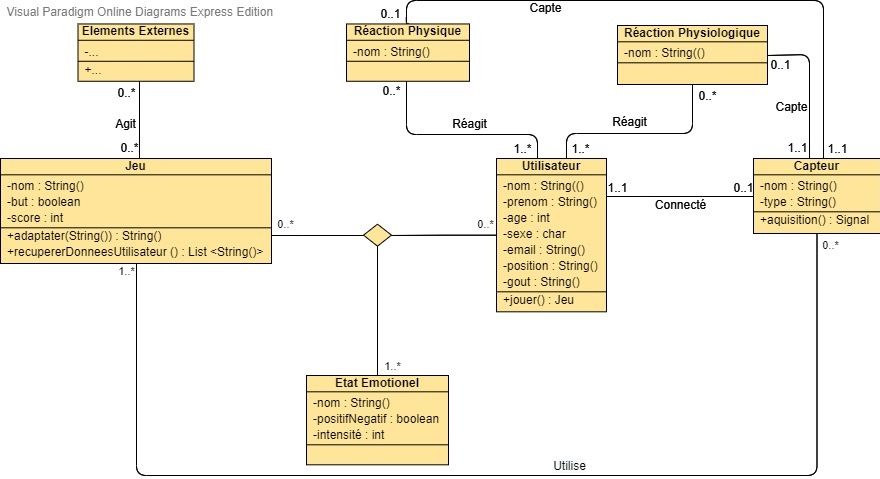
\includegraphics[scale=0.5]{../../include/ontologie_stage_cnam-v2-7.jpg}
			\caption{Ontologie d'un jeu pervasif prenant en compte l'état émotionnel du joueur}
			\label{fig:modele}
		\end{figure}
		Le diagramme de la Figure \ref{fig:modele} représente notre contribution pour une modélisation pour le projet.
		Dans cette représentation, nous avons apporté une première contribution à notre problématique.
		Nous nous sommes intéressés tout particulièrement aux liens entre les différents éléments impliqués dans le traitement des donnés physiologiques et physiques pour la détection et la reconnaissance d'états émotionnels dans un jeu pervasif adaptable dynamiqument au contexte du joueur.\par
		Dans cette représentation, plusieurs concepts sont présentés.
		Chaque classe permet représente un élément essentiel dans la gestion de données générées par des capteurs.
		\begin{itemize}
			\item La classe \texttt{Jeu} englobe tout ce qui concerne le jeu pervasif que nous souhaitons concevoir;
			\item La classe \texttt{Utilisateur} représente le joueur;
			\item La classe \texttt{Etat Emotionnel} représente l'état émotionnel du joueur. Cet état sera déduit par des élgorithmes comme ceux présentés dans \cite{gal_2019, gal_et_al._2020};
			\item La classe \texttt{Réaction Physique} représente les réactions physiques de l'utilisateur;
			\item La classe \texttt{Réaction Physiologique} représente les réactions physiologiques de l'utilisateur;
			\item La classe \texttt{Capteur} représente les capteurs utilisés le jeu pour acquérir des métriques physiques et/ou physiologiques d'un utilisateur;
			\item La classe \texttt{Elements Externes} représente tous les éléments de l'environnement du jeu;=.
		\end{itemize}\par
		Une relation ternaire existe entre \texttt{Jeu}, \texttt{Etat Emotionel} et \texttt{Utilisateur}.
		Cette relation est dûe au lien très fort qu'il existe entre ces trois classes.
		En effet, le jeu entraine un état émotionnel qui est expérimenté par l'utilisateur lorsqu'il joue à ce jeu.
		Cette notion est notamment expliquée dans \cite{calvo_et_al._2015}.
		La classe \texttt{Capteur} a une relation avec \texttt{Utilisateur} car c'est l'utilisateur qui porte le ou les capteurs.
		Ce ou ces capteurs permettent d'acquérir des métriques sur une (ou plusieurs) réaction physique ou physiologique (réciproquement représentés par les classes \texttt{Réaction Physique} et/ou \texttt{Réaction Physiologique}) de l'utilisateur  (détaillés dans \cite{shu_et_al._2018}).
		Ces métriques sont utilisés par le jeu pour en déduir l'état émotionnel courant du joueur (voir la Section \ref{sec:eda}).
		La classe \texttt{Elements Externes} représente tous les éléments liés à l'environnement qui seront pris en compte par le jeu.
		Cette classe permet simplement de rappeler que d'autres éléments que l'état émotionnel seront à considérés dans de futurs travaux.
		Cependant, nous ne détaillons pas ce composant ici car notre contribution vise à répondre à la problématique liée aux données générées par les capters physiologiques.
	\subsection{Difficultés rencontrées}\label{sec:difficultes}
		L'ontologie que je présente dans ce rapport à la Figure \ref{fig:modele} n'est pas le résultat définitif du modèle conceptuel que nous cherchons à élaborer.
		Lors de l'élaboration de cette cette ontologie, plusieurs essais et plusieurs versions différentes ont été proposés.
		Cependant, le modèle était toujours incohérent, il manquait de substance et présentait plusieurs niveaux d'abstraction qui ne devait pas figurer sur un même modèle. 
		Cela peut s'expliquer de différentes manières. 
		L'une des explications est que je me suis lancée trop rapidement, selon moi, dans la conception de cette ontologie.
		Je pense que je ne maîtrisais pas encore assez bien le sujet, l'objectif et la problématique de notre projet.
		De ce fait, j'ai eu tendance à mélanger les niveaux d'abstraction.
		Une autre explication est qu'avec les différentes approches que je lisais parallèlement à la construction de cette ontologie, j'ai voulu retranscrire dans ce modèle tout ce que j'assimilais au fil de mes lectures.
		Ce qui faisait que j'ajoutais à ce modèle des éléments superflus.
		Une dernière explication est que je manquais de recul sur mon travail.
		Dès que je terminais une version de l'ontologie et que celle-ci n'était pas correcte, je commençait une nouvelle version.
		Je ne laissais pas de temps de repos entre chaque nouvel essai.\par
		Pour toutes ces raisons que nous avons décidé de changer de point de vue et de problématique.
		Nous avons décidé de revenir, si possible, plus tard à l'ontologie.
	\subsection{Bilan}\label{sec:modelbilan}
		Le bilan que je tire de cet exercice de modélisation est que malgré cet échec d'aboutir à une ontologie livrable, j'ai pu, d'une part, mieux comprendre la problématique liée au projet et à la conception de modèles.
		Et d'autre part, j'ai pu me rendre compte de l'étendue des difficultés qu'il  était possible de rencontrer dans ce genre d'exercice.
		Par exemple, lors de la conception de cette ontologie, je me suis retrouvée à mélanger plusieurs niveaux d'abstraction, ce qui la rendait peu compréhensible et invalide.
		Je me suis aussi rendu compte qu'il fallait beaucoup de patience et d'entraînement pour concevoir un tel modèle.
		Aujourd'hui, je comprends mieux les enjeux de tels modèles.
		A l'avenir je pourrais réaliser des modèles de meilleure qualité grâce à cette expérience.\par
		La réalisation de cette ontologie nous a permis de réorienter notre objectif de recherche.
		Nous nous sommes dirigés vers l'implémentation d'une solution pour la gestion des données générées par les capteurs physiologiques.



\bibliographystyle{abbrv}
\bibliography{../../include/biblio}

\section{Liste des capteurs}\label{ann:capteursed}
\end{document}